\subsection{Evaluaci\'on final de desempe\~no del software 3}

    Para la evaluaci\'on final del simulador, esta vez no fue necesario del manejo en espacios
        mucho m\'as grandes en cuanto al tama\~no del lienzo, sino a entornos m\'as acordes a la realidad
        donde hay m\'as posibilidad de encontrar alg\'un fallo o generaci\'on de rutas u obst\'aculos fuera
        de lo originalmente planteado. Un ejemplo es la generaci\'on de una ruta para llegar de un
        punto a otro dentro del circuito del Instituto Polit\'ecnico Nacional, en el cual se puso a prueba
        el simulador para poder encontrar la ruta dentro de una locaci\'on a otra en este circuito y
        comprobar c\'omo es que el simulador se comportaba uniendo tanto el cargado de mapas, como
        de la generaci\'on de las rutas a trav\'es del Physarum.
    \vskip 0.5cm
    En las Figuras \ref{fig:90} y \ref{fig:91}, se muestran algunos de los datos recopilados con los que fue evaluado el
    software en la generaci\'on de rutas.
    \vskip 0.5cm
    %figura
    \begin{figure}[htbp]
        \centering
        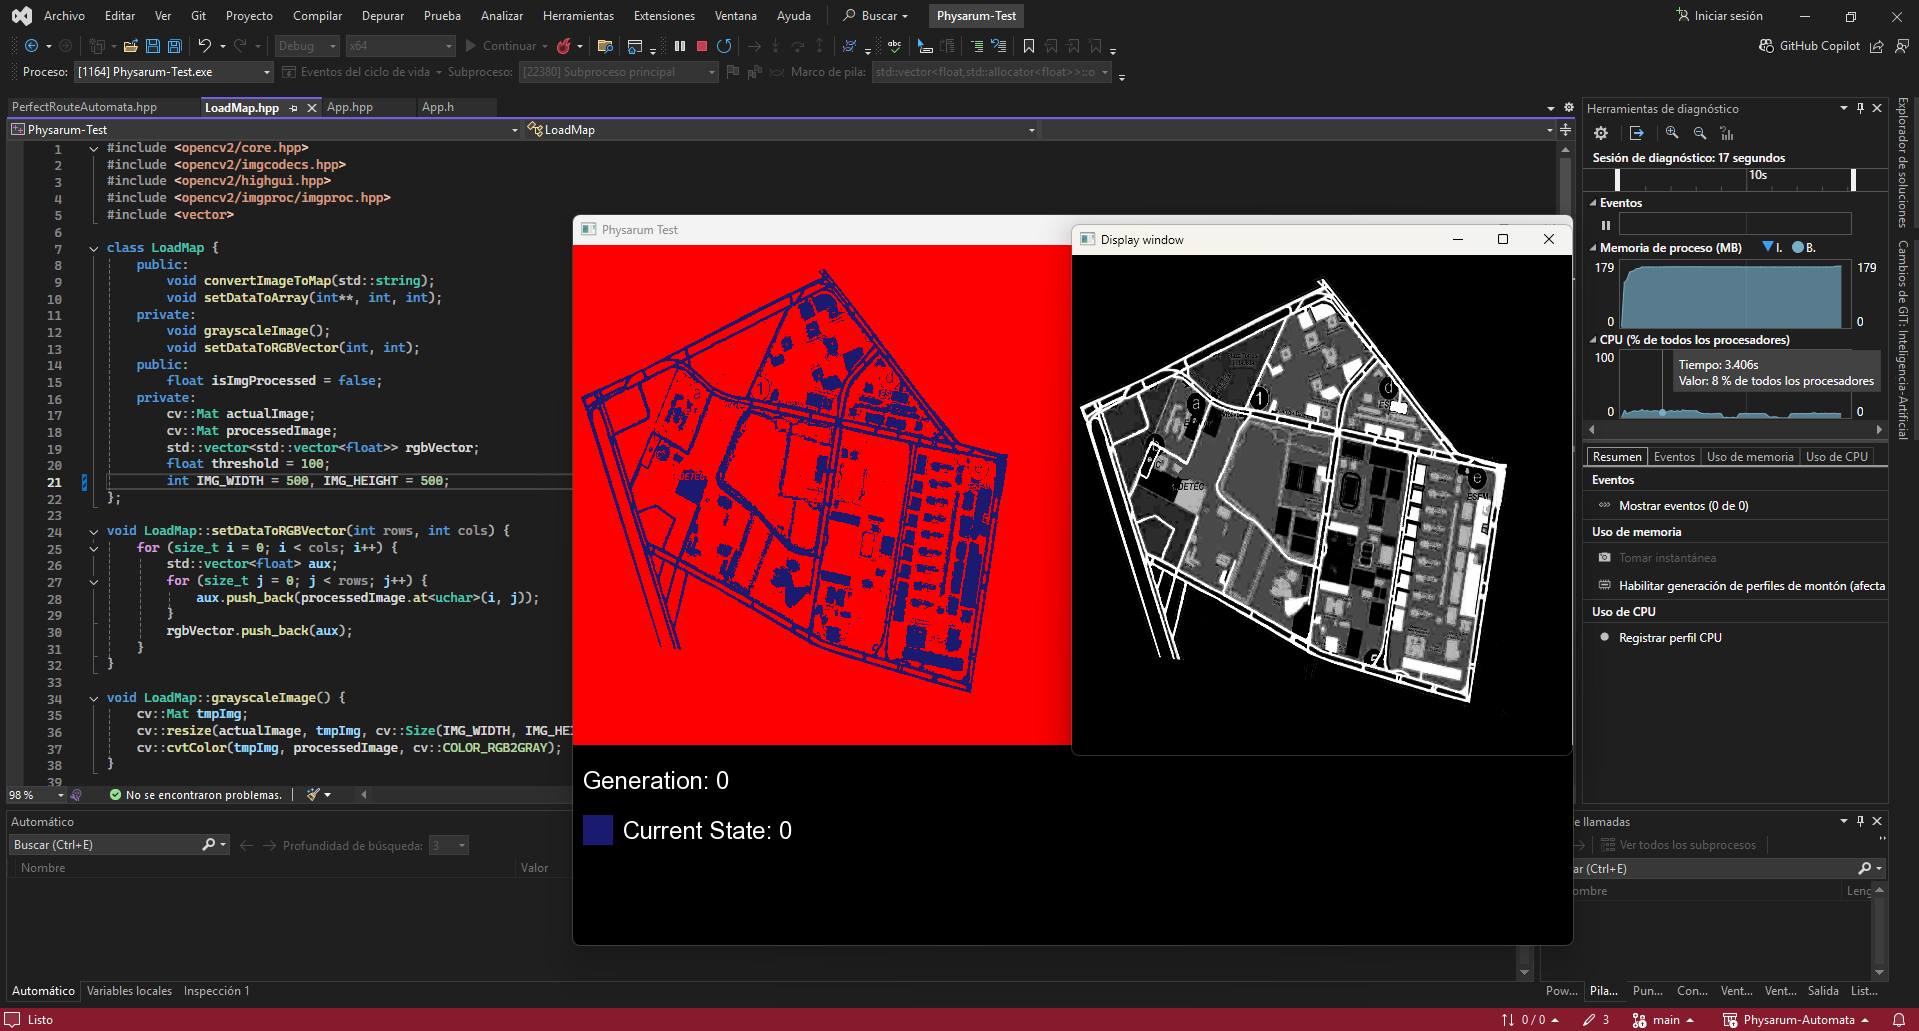
\includegraphics[width=0.5\textwidth]{./images/Pruebas/simulador/image090.png}
        \caption{An\'alisis del simulador sobre el porcentaje de uso del procesador.}
        \label{fig:90}
    \end{figure}
    \vskip 0.5cm
    %figura
    \begin{figure}[htbp]
        \centering
        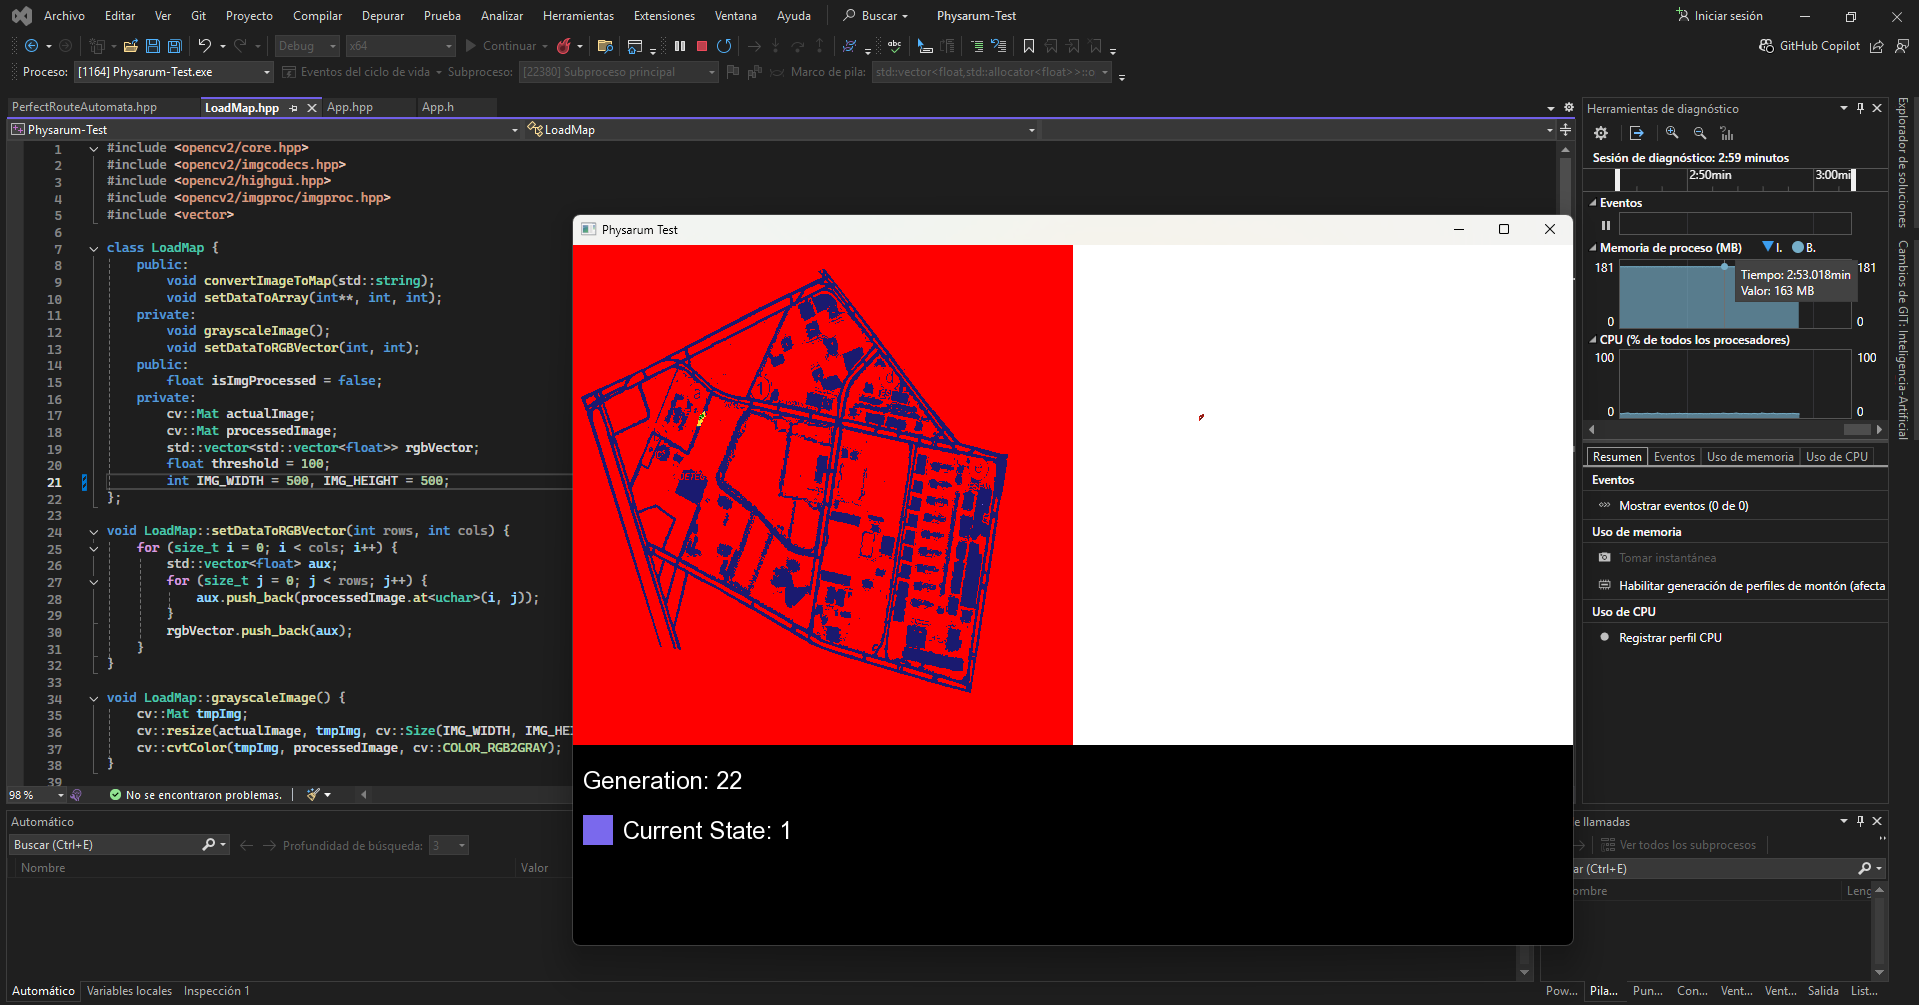
\includegraphics[width=0.5\textwidth]{./images/Pruebas/simulador/image091.png}
        \caption{An\'alisis del uso de memoria por parte del simulador durante la ejecuci\'on del programa en la
        generaci\'on de rutas.}
        \label{fig:91}
    \end{figure}
    \vskip 0.5cm
    Con la informaci\'on recopilada, podemos darnos cuenta de que mientras m\'as grande el lienzo
        y la imagen que se le sea proporcionada al simulador, el programa tiene un uso mayor del
        procesador, as\'i como del uso de la memoria debido a que en ese momento hay muchos m\'as
        p\'ixeles que dibujar en pantalla, as\'i como tambi\'en el tama\~no del arreglo se vuelve mucho m\'as
        grande, lo que hace complicado y m\'as tardado la evaluaci\'on y la generaci\'on de la ruta debido
        a que no se est\'a lo suficientemente optimizado para espacios mucho m\'as grandes.